% TikZ: SysPlug System Overview Diagram
\begin{figure}[h]
\centering
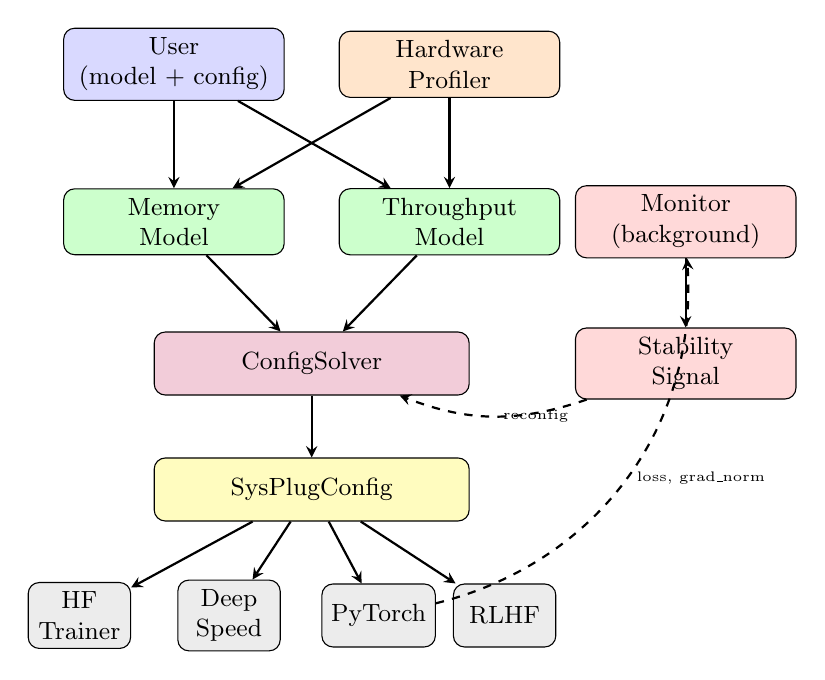
\begin{tikzpicture}[
  box/.style={draw, rectangle, rounded corners, minimum width=2.8cm, minimum height=0.8cm,
              align=center, font=\small},
  arrow/.style={->, thick, >=stealth},
  every node/.style={font=\small}
]

% Input layer
\node[box, fill=blue!15] (user) at (0, 0) {User\\(model + config)};
\node[box, fill=orange!20] (hw) at (3.5, 0) {Hardware\\Profiler};

% Core models
\node[box, fill=green!20] (mem) at (0, -2) {Memory\\Model};
\node[box, fill=green!20] (tput) at (3.5, -2) {Throughput\\Model};

% Solver
\node[box, fill=purple!20, minimum width=4cm] (solver) at (1.75, -3.8) {ConfigSolver};

% Output
\node[box, fill=yellow!25, minimum width=4cm] (config) at (1.75, -5.4) {SysPlugConfig};

% Monitor path
\node[box, fill=red!15] (monitor) at (6.5, -2) {Monitor\\(background)};
\node[box, fill=red!15] (stability) at (6.5, -3.8) {Stability\\Signal};

% Integrations
\node[box, fill=gray!15, minimum width=1.3cm] (hf) at (-1.2, -7) {HF\\Trainer};
\node[box, fill=gray!15, minimum width=1.3cm] (ds) at (0.7, -7) {Deep\\Speed};
\node[box, fill=gray!15, minimum width=1.3cm] (pt) at (2.6, -7) {PyTorch};
\node[box, fill=gray!15, minimum width=1.3cm] (rlhf) at (4.2, -7) {RLHF};

% Arrows
\draw[arrow] (user) -- (mem);
\draw[arrow] (hw) -- (mem);
\draw[arrow] (hw) -- (tput);
\draw[arrow] (user) -- (tput);
\draw[arrow] (mem) -- (solver);
\draw[arrow] (tput) -- (solver);
\draw[arrow] (solver) -- (config);

\draw[arrow] (config) -- (hf);
\draw[arrow] (config) -- (ds);
\draw[arrow] (config) -- (pt);
\draw[arrow] (config) -- (rlhf);

\draw[arrow] (monitor) -- (stability);
\draw[arrow, dashed] (stability) to[bend left=20] node[right,font=\tiny]{reconfig} (solver);

% Training loop feedback
\draw[arrow, dashed] (pt) to[bend right=40] node[right,font=\tiny]{loss, grad\_norm} (monitor);

\end{tikzpicture}
\caption{SysPlug system overview. Solid arrows indicate configuration flow;
dashed arrows indicate online monitoring feedback.}
\label{fig:overview}
\end{figure}
